\chapter{稳态热传导}
\thispagestyle{empty}
\section{导热基本定律——傅立叶定律}
\subsection{温度场}

\noindent \textbf{1.温度场的定义}

\defination[温度场]
物体在各个时刻各点的温度所组成的集合称为\dy[温度场]{WDC}。
\vspace*{1em}

\noindent \textbf{2.表示方法}\\
温度场是空间(空间坐标$x, y, z$)和时间$\tau$的函数,直角坐标系中表示为
\begin{align}
	T = T (x, y, z, \tau)
\end{align}

\noindent \textbf{3.温度场的分类}
\begin{equation*}
	\mbox{温度场的分类}\,
	\begin{cases}
		\,\mbox{按时间分类}\,
		\begin{cases}
			\, \mbox{\makecell[c]{\dy[稳态温度场]{WTWDC}\\(\dy[定常温度场]{DCWDC})}}\quad \mbox{物体的温度场不随时间而变} \quad \xrightarrow{\scriptsize \,\,\mbox{热传导} \, \,} \quad \mbox{\makecell[c]{\dy[稳态热传导]{WTRCD}\\ (\dy[稳态导热]{WTDR})}} \\[2em]
			\, \mbox{\makecell[c]{\dy[非稳态温度场]{FWTWDC}\\(\dy[非定常温度场]{FDCWDC})}}\quad \mbox{物体的温度场随时间而变} \quad \xrightarrow{\scriptsize \,\,\mbox{热传导} \, \,} \quad \mbox{\makecell[c]{\dy[非稳态热传导]{FWTRCD} \\(\dy[非稳态导热]{FWTDR})}} 
		\end{cases} \\[5em]
		\,\mbox{按空间分类}\,
		\begin{cases}
			\, \mbox{\makecell[c]{\dy[一维温度场]{YWWDC}}}\quad \mbox{物体的温度场仅在一个空间方向变化} \quad \xrightarrow{\scriptsize \,\,\mbox{热传导} \, \,} \quad \mbox{\makecell[c]{\dy[一维热传导]{YWRCD}\\ (\dy[一维导热]{YWDR})}} \\[2em]
			\, \mbox{\makecell[c]{\dy[多维温度场]{DWWDC}}}\quad \mbox{物体的温度场在两(三)个空间方向变化} \quad \xrightarrow{\scriptsize \,\,\mbox{热传导} \, \,} \quad \mbox{\makecell[c]{\dy[多维热传导]{DWRCD} \\(\dy[多维导热]{DWDR})}} 
		\end{cases}
	\end{cases}
\end{equation*}
\begin{itemize}
	\item 稳态温度场\\
	若物体的温度场不随时间而变,则称为\dy[稳态温度场]{WTWDC},或称\dy[定常温度场]{DCWDC};相应的热传导称为\dy[稳态热传导]{WTRCD},简称\dy[稳态导热]{WTDR}。
	\begin{align}
		T = T(x, y, z)
	\end{align}
\end{itemize}

\noindent \textbf{4.温度的方向导数和温度梯度}
\begin{itemize}
	\item 温度沿$ \vec{l} = (\cos \alpha, \cos \beta, \cos \gamma)$的方向导数为
	\begin{align}
		\dfrac{\partial T}{\partial \vec{l}} = \dfrac{\partial T}{\partial x} \cos \alpha + \dfrac{\partial T}{\partial y}\cos \beta + \dfrac{\partial T}{\partial z} \cos \gamma 
	\end{align}

	\item 温度梯度为
	\begin{align}
		\nabla T = \dfrac{\partial T}{\partial x} \vec{i} + \dfrac{\partial T}{\partial y} \vec{j} + \dfrac{\partial T}{\partial z} \vec{k}
	\end{align}
	
	\item \textbf{在温度梯度的方向上,温度的方向导数取最大值。}
\end{itemize}

\noindent \textbf{5. 等温面和等温线}

	三维物体内同一时刻所有温度相同的点的集合称为\dy[等温面]{DWM}。
	
	一个平面与等温面的交线称为\dy[等温线]{DWX}。
	
	\textbf{温度梯度矢量与等温面(线)垂直。}
	\vspace*{1em}

\subsection{导热基本定律}

\vspace*{-1.5em}\theorem[导热基本定律]

任意时刻,各向同性的连续介质中任意地点的热流密度与该点的温度梯度大小成正比,方向相反,这一定律称为\dy[傅立叶定律]{FLYDL},又称为\dy[导热基本定律]{DRJBDL}。
\begin{align}
	\vec{q} = - \lambda \nabla T
	\label{导热基本定律}
\end{align}
其中,
\begin{enumerate}[\hspace*{1.5em}]
	\item $\vec{q}$ \quad 热流密度,单位时间通过单位面积传递的热量,单位:J/(s $\cdot \text{m}^2$)\vspace*{-0.5em}
	\item $\lambda$ \quad 导热系数(热导率),单位:J/(s$\cdot$m$\cdot$K)\vspace*{-0.5em}
	\item $T$ \quad 热力学温度,单位:K\vspace*{-0.5em}
\end{enumerate}
公式\eqref{导热基本定律}中的负号表示热量的传递方向指向温度降低的方向,这是热力学第二定律所要求的。
\vspace*{1em}

\subsection{导热系数}
	傅立叶定律表达式$\vec{q} = -\lambda \nabla T$中出现肋一个新系数$\lambda$,称为\dy[导热系数]{DRXS},或称\dy[热导率]{RDL},单位为J/(s$\cdot$m$\cdot$K),导热系数是物质的热物理性质\footnote{热物理性质包括热力学性质(如温度、压强、比容、比热容等)和输运系数(如导热稀释、粘性系数、质扩散系数等)}之一。
	
\begin{equation*}
	\mbox{影响因素}\,
	\begin{cases}
		\, \mbox{物体的种类}\\
		\, \mbox{物体的温度}
	\end{cases}
	\quad \quad \quad \quad 
	\mbox{获取导热系数的方法}\,
	\begin{cases}
		\, \mbox{专门实验测得}\\
		\, \mbox{已有图表查得}
	\end{cases}
\end{equation*}

固体、液体、气体导热系数差异较大的原因:导热机理不同
\begin{itemize}
	\item 固体的导热机理:自由电子迁移和晶格振动\vspace*{-0.5em}
	\begin{itemize}
		\item 金属的导热系数大于非金属的导热系数(钻石和硅除外)\vspace*{-0.5em}
		\item 金属地点导热系数排序和电导率排序完全相同(常温下:银>铜>金>铝>铁)\vspace*{-0.5em}
		\item 非金属材料中,导热系数很低的材料可用作隔热材料\vspace*{-0.5em}
		\item 温度升高时,金属的导热系数一般减小,两种金属形成合金,导热系数降低
	\end{itemize}
	\item 液体的导热机理:\vspace*{-0.5em}
	\begin{itemize}
		\item 一般而言,液体的导热系数介于固体和气体的导热系数之间,液态金属除外\vspace*{-0.5em}
		\item 在非金属液体中,水的导热系数最大\vspace*{-0.5em}
		\item 温度升高,液体的导热系数一般减小,水例外(非单调)
	\end{itemize}
	\item 气体的导热原理:分子碰撞\vspace*{-0.5em}
	\begin{itemize}
		\item 氢气和氦气具有比其他气体高得多的导热系数,因而常作为气冷介质\vspace*{-0.5em}
		\item 温度升高时,所有气体的导热系数均增大
	\end{itemize}
\end{itemize}

\subsection{工程导热材料按导热系数的分类}
\noindent \textbf{1. 均匀各项同性材料的导热系数}

在同一温度下,材料中不同地点以及同一地点的不同方向上的导热系数相同。
\vspace*{1em}

\noindent \textbf{2.工程导热材料}\vspace*{-0.5em}
\begin{itemize}
	\item 均匀各向同性材料,如图\ref{工程导热材料}(a).\vspace*{-0.5em}
	\item 均匀各向异性材料\ref{工程导热材料}(b).\vspace*{-0.5em}
	\item 不均匀各向同性材料\ref{工程导热材料}(c).\vspace*{-0.5em}
	\item 不均匀各向异性材料\ref{工程导热材料}(d).
\end{itemize}

\begin{figure}[!htb]
	\centering
	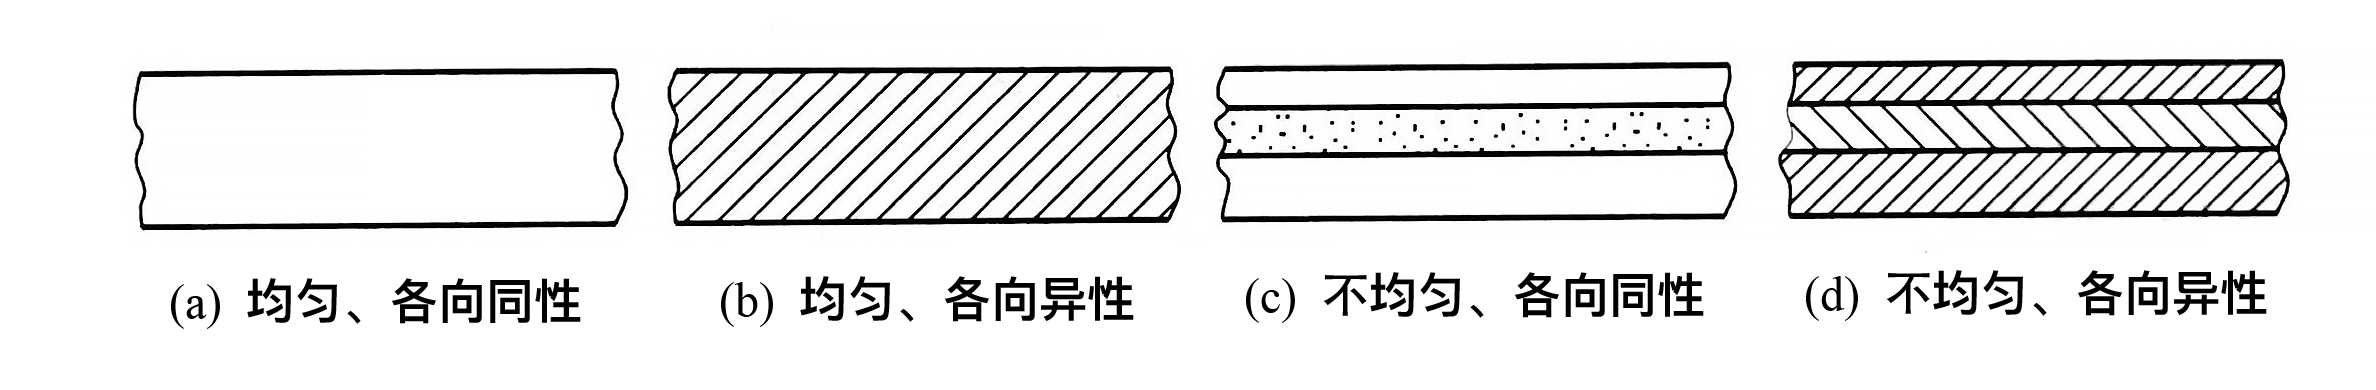
\includegraphics[width=0.9\linewidth]{pic/传热材料分类.jpg}
	\vspace*{-2em}
	\caption{工程导热材料}
	\label{工程导热材料}
\end{figure}

\section{导热问题的数学描述}
\subsection{导热微分方程}
\begin{equation*}
	\begin{cases}
		\, \mbox{理论基础}
		\begin{cases}
			\, \mbox{傅立叶定律}\\
			\, \mbox{能量守恒定律}
		\end{cases}\\[2em]
		\, \mbox{前提假设}
		\begin{cases}
			\, \mbox{研究对象是各向同性的连续介质}\\
			\, \mbox{密度、比热容、导热系数均已知}\\
			\, \mbox{物体内可以具有均匀分布的热源}
		\end{cases}
	\end{cases}
\end{equation*}
在导热物体内任意取一微元体,根据能量守恒定律,在$\d \tau$时间内,有
\vspace*{-0.5em}
\begin{equation*}
	\mbox{\textbf{净导入微元体的热量}} \, \bm{+} \, \mbox{\textbf{微元体内热源生成的热量}} \, \bm{=} \, \mbox{\textbf{微元体热力学能的增量}}
\end{equation*}
\vspace*{-1em}
\begin{figure}[!htb]
	\centering
	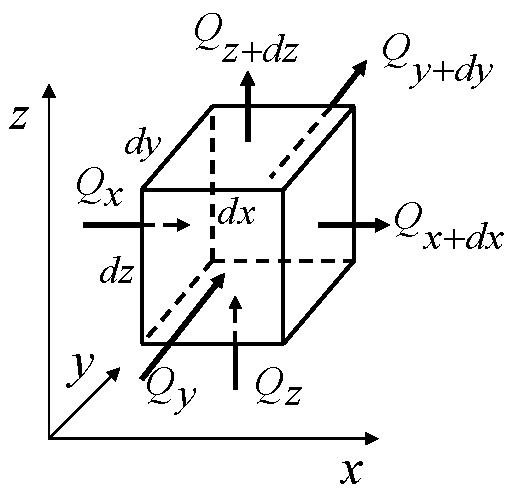
\includegraphics[width=0.3\linewidth]{pic/导热方程.pdf}
	\vspace*{-1.5em}
	\caption{微元体的导热过程}
	\label{导热过程}
\end{figure}
即
\begin{align}
	\delta Q_1 + \delta Q_2 = \delta U
\end{align}

根据傅立叶定律,$\d \tau $时间内$x$方向导入微元体的净热量为
\begin{align}
	\delta Q_x  &= Q_x - \left(Q_x + \dfrac{\partial Q_x}{\partial x} \,\d x\right) = - \dfrac{\partial Q_x}{\partial x}\,\d x = - \dfrac{\partial (q_x \,\d y \d z \d \tau)}{\partial x} \, \d x \notag \\
	& = - \dfrac{\partial }{\partial x}\left(- \lambda \dfrac{\partial t}{\partial x}\, \d y \d z \d \tau \right)\, \d x = \dfrac{\partial }{\partial x}\left(\lambda \dfrac{\partial t}{\partial x}\right)\, \d V  \d \tau
\end{align}
同理可得,$y, z$方向导入微元体的净热量为
\begin{align}
	\delta Q_y = \dfrac{\partial }{\partial y}\left(\lambda \dfrac{\partial t}{\partial y}\right)\, \d V  \d \tau\\[0.5em]
	\delta Q_z = \dfrac{\partial }{\partial z}\left(\lambda \dfrac{\partial t}{\partial z}\right)\, \d V  \d \tau
\end{align}
则
\begin{align}
	\delta Q_1 = \delta Q_x + \delta Q_y + \delta Q_z = \left[\dfrac{\partial }{\partial x}\left(\lambda \dfrac{\partial t}{\partial x}\right) + \dfrac{\partial }{\partial y}\left(\lambda \dfrac{\partial t}{\partial y}\right) + \dfrac{\partial }{\partial z}\left(\lambda \dfrac{\partial t}{\partial z}\right) \right] \, \d V \d \tau
\end{align}


$\bm{\d \tau}$\textbf{时间内的微元体内热源生成的热量}
\begin{align}
	\delta Q_2 = \dot{\varPhi}\, \d V \d \tau
\end{align}
其中,$\dot{\varPhi}$为\dy[热源强度]{RYQD},导热物体单位体积单位时间内产生的热量。
\vspace*{1em}

$\bm{\d \tau}$\textbf{时间内微元体热力学能的增量}
\begin{align}
	\delta U = \rho c \dfrac{\d t}{\d \tau}\, \d V \d \tau
\end{align}
其中,\vspace*{-0.5em}
\begin{enumerate}[\hspace*{1.5em}]
	\item $\rho$ \quad 物质密度\vspace*{-0.5em}
	\item $c$ \quad 比热容\vspace*{-0.5em}
\end{enumerate}

从而得到直角坐标系中\textbf{三维非稳态导热微分方程的一般形式}为
\begin{align}
	\rho c \dfrac{\partial t}{\partial \tau} = \dfrac{\partial }{\partial x}\left(\lambda \dfrac{\partial t}{\partial x}\right) + \dfrac{\partial }{\partial y}\left(\lambda \dfrac{\partial t}{\partial y}\right) + \dfrac{\partial }{\partial z}\left(\lambda \dfrac{\partial t}{\partial z}\right) + \dot{\varPhi}
\end{align}
对于不同的情况,可以做不同的简化
\begin{enumerate}[\hspace*{2em}\textbf{情形} 1  ]
	\item \textbf{导热系数为常数}
	\begin{align}
		\dfrac{\partial t}{\partial \tau} = a \left(\dfrac{\partial^2 t}{\partial x^2} + \dfrac{\partial^2 t}{\partial y^2} + \dfrac{\partial^2 t}{\partial z^2}\right) + \dfrac{\dot{\varPhi}}{\rho c} = a \nabla^2 t + \dfrac{\dot{\varPhi}}{\rho c}
	\end{align}
	其中,$a = \dfrac{\lambda}{\rho c}$称为\dy[热扩散系数]{RKSXS}或\dy[热扩散率]{RKSL},又称\dy[导温系数]{DWXS},单位为$\text{m}^2$/s
	\vspace*{0.5em}
	
	\item \textbf{导热系数为常数、无内热源}
	\begin{align}
		\dfrac{\partial t}{\partial \tau} = a \nabla^2 t
	\end{align}

	\item \textbf{导热系数为常数、达到稳态}
	\begin{align}
		\lambda \nabla^2 t + \dot{\varPhi} = 0
	\end{align}

	\item \textbf{导热系数为常数、达到稳态、无内热源}
	\begin{align}
		\lambda \nabla^2 t  = 0
		\label{Lp}
	\end{align}
	公式\eqref{Lp}称为\dy[Laplace方程]{Laplace}。
	
	\item \textbf{导热系数为常数、达到稳态、无内热源、一维}
	\begin{align}
		\dfrac{\d^2 t}{\d x^2} = 0
	\end{align}

	\item \textbf{圆柱坐标系中导热系数为常数、达到稳态、无内热源}
	\begin{align}
		\dfrac{\partial^2 t}{\partial \tau^2} + \dfrac{1}{r} \dfrac{\partial t}{\partial \tau} + \dfrac{1}{r^2} \dfrac{\partial^2 t}{\partial \theta^2} + \dfrac{\partial^2 t}{\partial z^2} = 0 
	\end{align}

	\item \textbf{圆球坐标系中导热系数为常数、达到稳态、无内热源}
	\begin{align}
		\dfrac{1}{r} \dfrac{\partial }{\partial r^2}(rt) + \dfrac{1}{r^2\sin \theta} \dfrac{\partial }{\partial \theta} \left(\sin \theta \dfrac{\partial t}{\partial \theta}\right) + \dfrac{1}{r^2 \sin \theta}\dfrac{\partial^2 t}{\partial \varphi^2}= 0 
	\end{align}
\end{enumerate}

\subsection{定解条件}
\begin{itemize}
	\item 几何条件 \quad 说明导热体的几何形状和大小,它确定了研究的空间区域,如:平壁或圆筒壁;厚度或直径等\vspace*{-0.5em}
	
	\item 物理条件 \quad 说明导热体的物理特征,包括材料的热物性和有无内热源等\vspace*{-0.5em}
	
	\item 初始条件\quad 给定过程初始时刻所研究范围(包括边界)内的温度分布\vspace*{-0.5em}
	
	\item 边界条件\quad 说明了所研究对象的边界上的传热情况\vspace*{-0.5em}
\end{itemize}

\begin{enumerate}[\textbf{第} 1 \textbf{类边界条件} ]
	\item \textbf{给定边界上的温度}
	\begin{itemize}
		\item 稳态导热\vspace*{-1em}
		\begin{align}
			t_\text{w} = C
		\end{align}
		\vspace*{-2em}
		\item 非稳态导热\vspace*{-1em}
		\begin{align}
			t_{\w} = f_1(\tau), \quad \tau > 0
		\end{align}
	\end{itemize}
	
	\item \textbf{给定边界上的热流密度}
	\begin{itemize}
		\item 稳态导热\vspace*{-1em}
		\begin{align}
			q_\w = - \lambda \left(\dfrac{\partial t}{\partial n}\right)_\w = C
		\end{align}
		\vspace*{-2em}
		\item 非稳态导热\vspace*{-1em}
		\begin{align}
			q_\w = - \lambda \left(\dfrac{\partial t}{\partial n}\right)_\w =f_2(\tau)\quad \tau > 0
		\end{align}
		\vspace*{-2em}
		\item 绝热边界条件\vspace*{-1em}
		\begin{align}
			q_\w = - \lambda \left(\dfrac{\partial t}{\partial n}\right)_\w = 0 \quad \Rightarrow \quad  \left(\dfrac{\partial t}{\partial n}\right)_\w = 0
		\end{align}
	\end{itemize}
	第二类边界条件相当于已知任何时刻物体边界面的温度梯度值
	
	\item 当导热物体表面与流体接触进行对流传热时,给定表面传热系数和周围流体的温度
	\begin{align}
		- \lambda \left(\dfrac{\partial t}{\partial n}\right)_\w = h(t_\w - t_{\text{f}})
	\end{align}
	\begin{itemize}
		\item 稳态导热\quad $t_\f , h$为已知常数\vspace*{-0.5em}
		\item 非稳态导热\quad $t_\f , h$为已知关于时间的函数\vspace*{-0.5em}
		\item $h \to \infty$,第三类边界条件变为第一类边界条件\vspace*{-0.5em}
		\item $h = 0$,第三类边界条件变为第二类边界条件中的绝热边界条件
	\end{itemize}
\end{enumerate}
\textbf{辐射边界条件}\quad 若导热物体表面与外界环境只发生辐射传热,则
\begin{align}
	- \lambda \left(\dfrac{\partial t}{\partial n}\right)_\w = \sigma \varepsilon (T_{\w}^4 - T_{\e}^4)
\end{align}
\hspace*{7em} $\sigma, \varepsilon, T_\w, T_\e$为斯忒藩—玻尔兹曼常数、导热物体发射率、导热物体表面温度、外界环境温度
\vspace*{1em}

\noindent \textbf{界面连续边界条件} \quad 对于发生在不均匀材料中的导热问题,采用分区方式求解,假定两种材料接触良好,在分界面上应满足如下条件
\begin{align}
	\begin{cases}
		\, t_{1} = t_2\\[0.5em]
		\, \left(- \lambda \dfrac{\partial t}{\partial n}\right)_1 = \left(- \lambda \dfrac{\partial t}{\partial n}\right)_2
	\end{cases}
\end{align}
\hspace*{8em} 其中下标1和2分别表示第一种材料和第二种材料。

\section{典型一维稳态导热的分析解}
\subsection{单层平壁的稳态导热}
单层平面壁的稳态导热如图\ref{平面壁}.
\begin{figure}[!htb]
\begin{minipage}{0.7\linewidth}
	\begin{enumerate}[\textbf{步骤} 1 ]
		\item \textbf{定解条件}
		\begin{itemize}
			\item 列出条件
			\begin{itemize}
				\item 几何条件
				\quad 单层平板厚度为$δ$
				\item 物理条件
				\quad $\rho ,c$已知,$λ$为常数,无内热源
				\item 初始条件
				\quad 稳态导热
				\item 边界条件
				\quad 第一类边界条件
			\end{itemize}
			\item 列出普适方程
			\begin{align*}
				\rho c \dfrac{\partial t}{\partial \tau} = \dfrac{\partial }{\partial x}\left(\lambda \dfrac{\partial t}{\partial x}\right) + \dfrac{\partial }{\partial y}\left(\lambda \dfrac{\partial t}{\partial y}\right) + \dfrac{\partial }{\partial z}\left(\lambda \dfrac{\partial t}{\partial z}\right) + \dot{\varPhi} 
			\end{align*}
			\item 列出定解条件
			\begin{align}
				\begin{cases}
					\, \dfrac{\d^2 t}{\d x^2} = 0 & t_1< t<t_2, 0< x< \delta\\
					\, x = 0, & t = t_1\\
					\, x = \delta, & t = t_2
				\end{cases}
			\end{align}
		\end{itemize}
	\end{enumerate}
\end{minipage}
\begin{minipage}{0.3\linewidth}
		\centering
		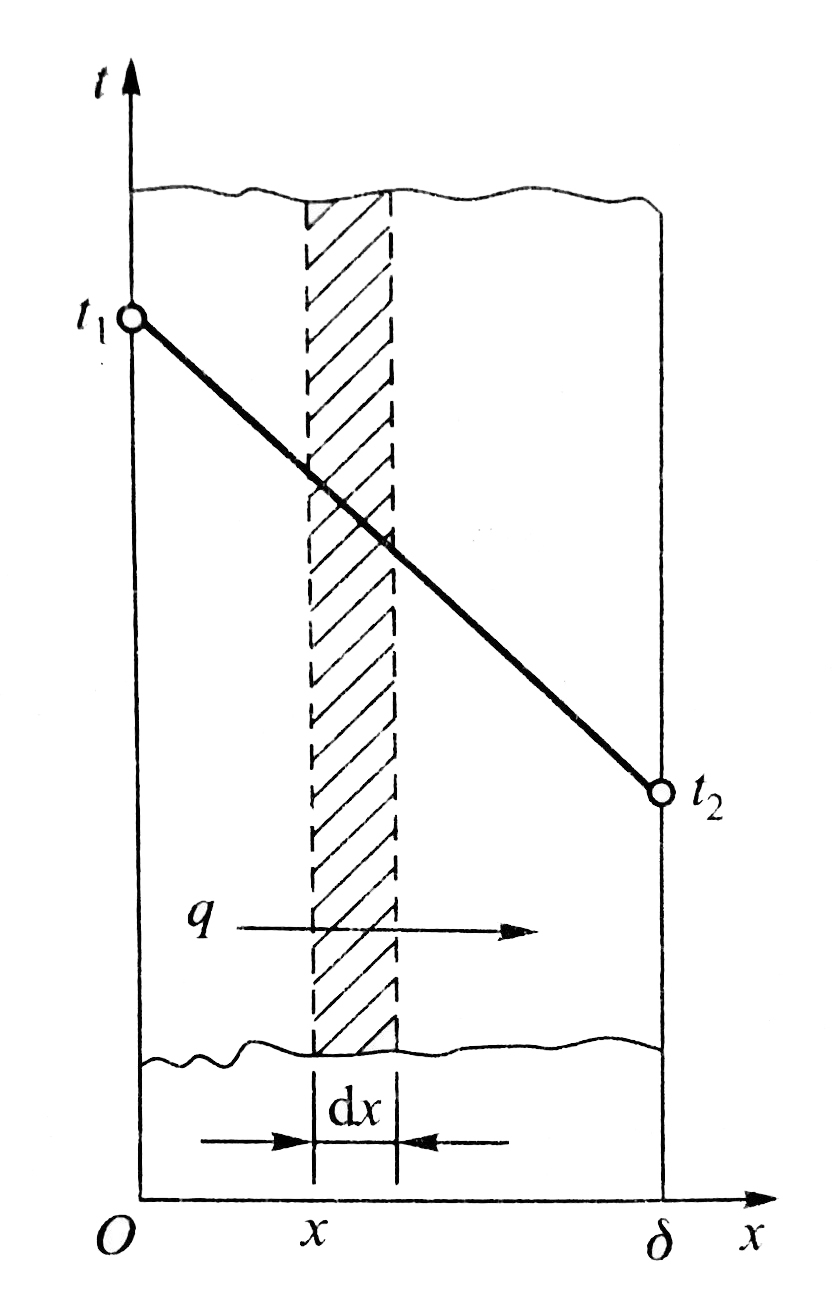
\includegraphics[width=\linewidth]{pic/平面壁.jpeg}
		\vspace*{-3em}
		\caption{平面壁的稳态导热}
		\label{平面壁}
	\end{minipage}
	\end{figure}

\begin{enumerate}[\textbf{步骤} 2 ]
	\item \textbf{求解方程}
	\begin{itemize}
		\item 通解
		\vspace*{-1.5em}
		\begin{align}
			t = C_1 x + C_2
		\end{align}
		\vspace*{-2.5em}
		\item 特解
		\vspace*{-1em}
		\begin{align}
			t = \dfrac{t_2 - t_1}{\delta} x + t_1
		\end{align}
		\vspace*{-2em}
	\end{itemize}
	
	\item \textbf{求出各个物理量}
	\begin{itemize}
		\item 热流密度
		\vspace*{-1em}
		\begin{align}
			q = - \lambda \dfrac{\d t}{\d x} = \dfrac{\lambda}{\delta}(t_1 - t_2) = \dfrac{\Delta t}{\delta / \lambda}
		\end{align}
		\vspace*{-2em}
	`	\item 热流量
		\vspace*{-1em}
		\begin{align}
			\varPhi = q A = \dfrac{\Delta t}{\delta /(A \lambda)}
		\end{align}
		\vspace*{-2em}
		\item 热阻
		\vspace*{-1em}
		\begin{align}
			R = \dfrac{\delta }{A \lambda}
		\end{align}
		\vspace*{-2em}
	\end{itemize}
\end{enumerate}

\subsection{多层平壁的稳态导热}
\vspace*{-3em}
	\begin{figure}[!htb]
		\begin{minipage}{0.7\linewidth}
			由多层不同材料的单层平壁组成的结构称为多层平壁,如图\ref{多平面壁}.
			
			假设:各层之间接触良好,可以近似认为结合面上各处温度相等
			\begin{enumerate}[\textbf{解法} 1]
				\item \textbf{对各层平壁分别求解}\\
				将单层传热的定解问一般化为
				\begin{align}
					\begin{cases}
						\, \dfrac{\d^2 t}{\d x^2} = 0, &  0< x< \delta\\
						\, t = t_1, & x = 0\\
						\, t = t_{n + 1}, & \displaystyle x = \sum_{i = 1}^n\delta_i
					\end{cases}
				\end{align}
				然后利用界面连续边界条件得到$t_2, t_3, \cdots , t_n$及各层温度分布和热流密度与热流量.
			\end{enumerate}
		\end{minipage}
	\begin{minipage}{0.3\linewidth}
		\centering
		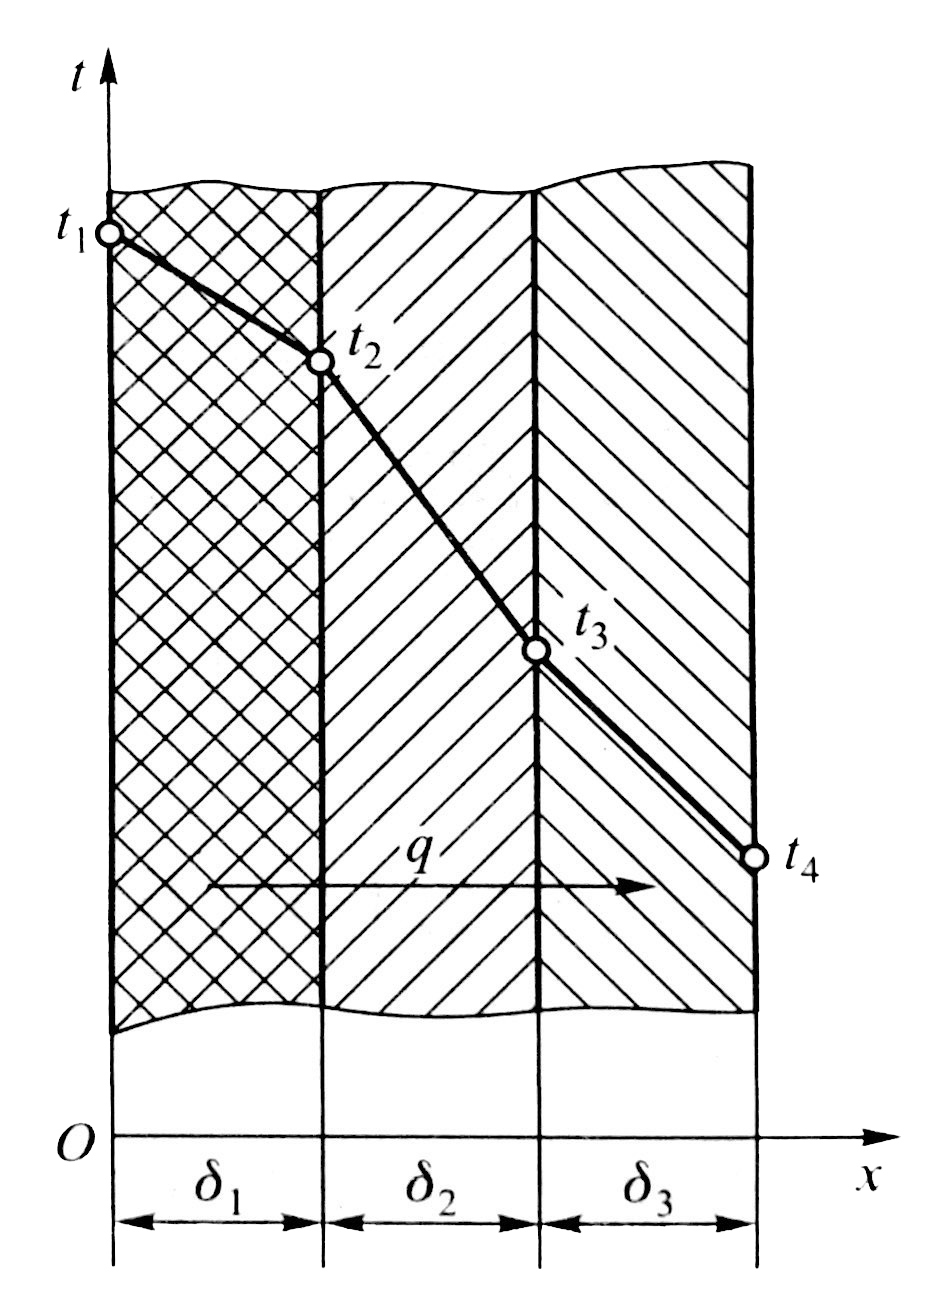
\includegraphics[width=\linewidth]{pic/多平面壁.jpeg}
		\vspace*{-3em}
		\caption{多层平面壁的稳态导热}
		\label{多平面壁}
	\end{minipage}
	\end{figure}
\vspace*{-2.5em}
	\begin{enumerate}[\textbf{解法} 2]
	\item \textbf{热阻分析方法}
	\begin{itemize}
		\item 热阻
		\begin{align}
			R = \sum_{ i =1}^n \dfrac{\delta_i }{A \lambda_i}
		\end{align}
		\vspace*{-2em}
		\item 热流密度
		\vspace*{-1em}
		\begin{align}
			q =  \dfrac{t_1 -t_{n+1}}{\displaystyle \sum_{ i =1}^n \dfrac{\delta_i }{A \lambda_i}}
		\end{align}
		\vspace*{-2em}
			\item 热流量
		\vspace*{-1em}
		\begin{align}
			q =  \dfrac{t_1 -t_{n+1}}{\displaystyle \sum_{ i =1}^n \dfrac{\delta_i }{ \lambda_i}}
		\end{align}
		\vspace*{-2em}
		\item 各层界面温度
		\vspace*{-1em}
		\begin{align}
			t_i = t_{i = 1} - q\dfrac{\delta_{i -1}}{\lambda_{i -1}}, \quad i = 1,2,3,\cdots,n
		\end{align}
		\vspace*{-2em}
	\end{itemize}
\end{enumerate}

\begin{figure}[!htb]
	\subsection{圆筒壁和球壁的稳态导热}
	\vspace*{-2em}
\end{figure}
\begin{figure}[!htb]
	\begin{minipage}{0.5\linewidth}
	\centering
	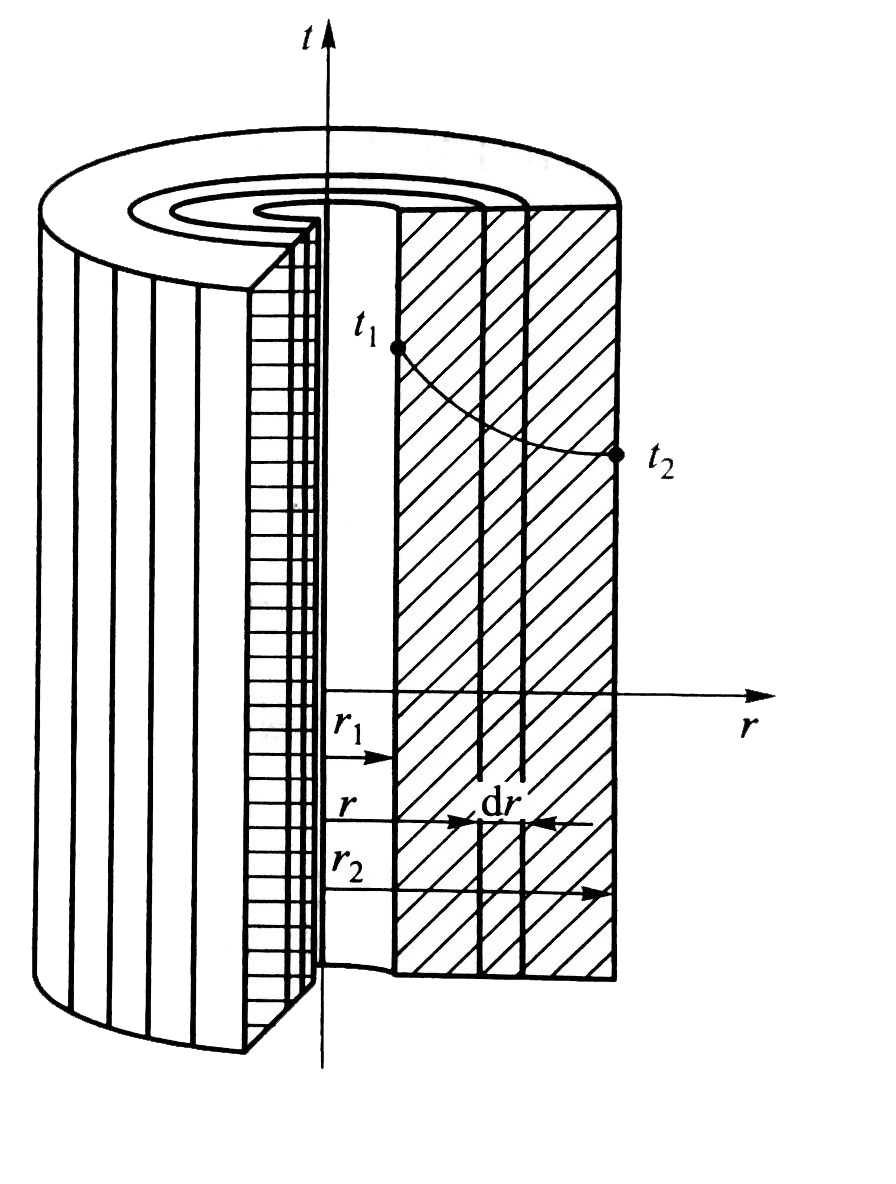
\includegraphics[width=0.5\linewidth]{pic/圆筒壁.jpeg}
	\vspace*{-2em}
	\caption{圆筒壁的稳态导热}
	\label{圆筒壁}
	\end{minipage}
	\begin{minipage}{0.5\linewidth}
		\centering
		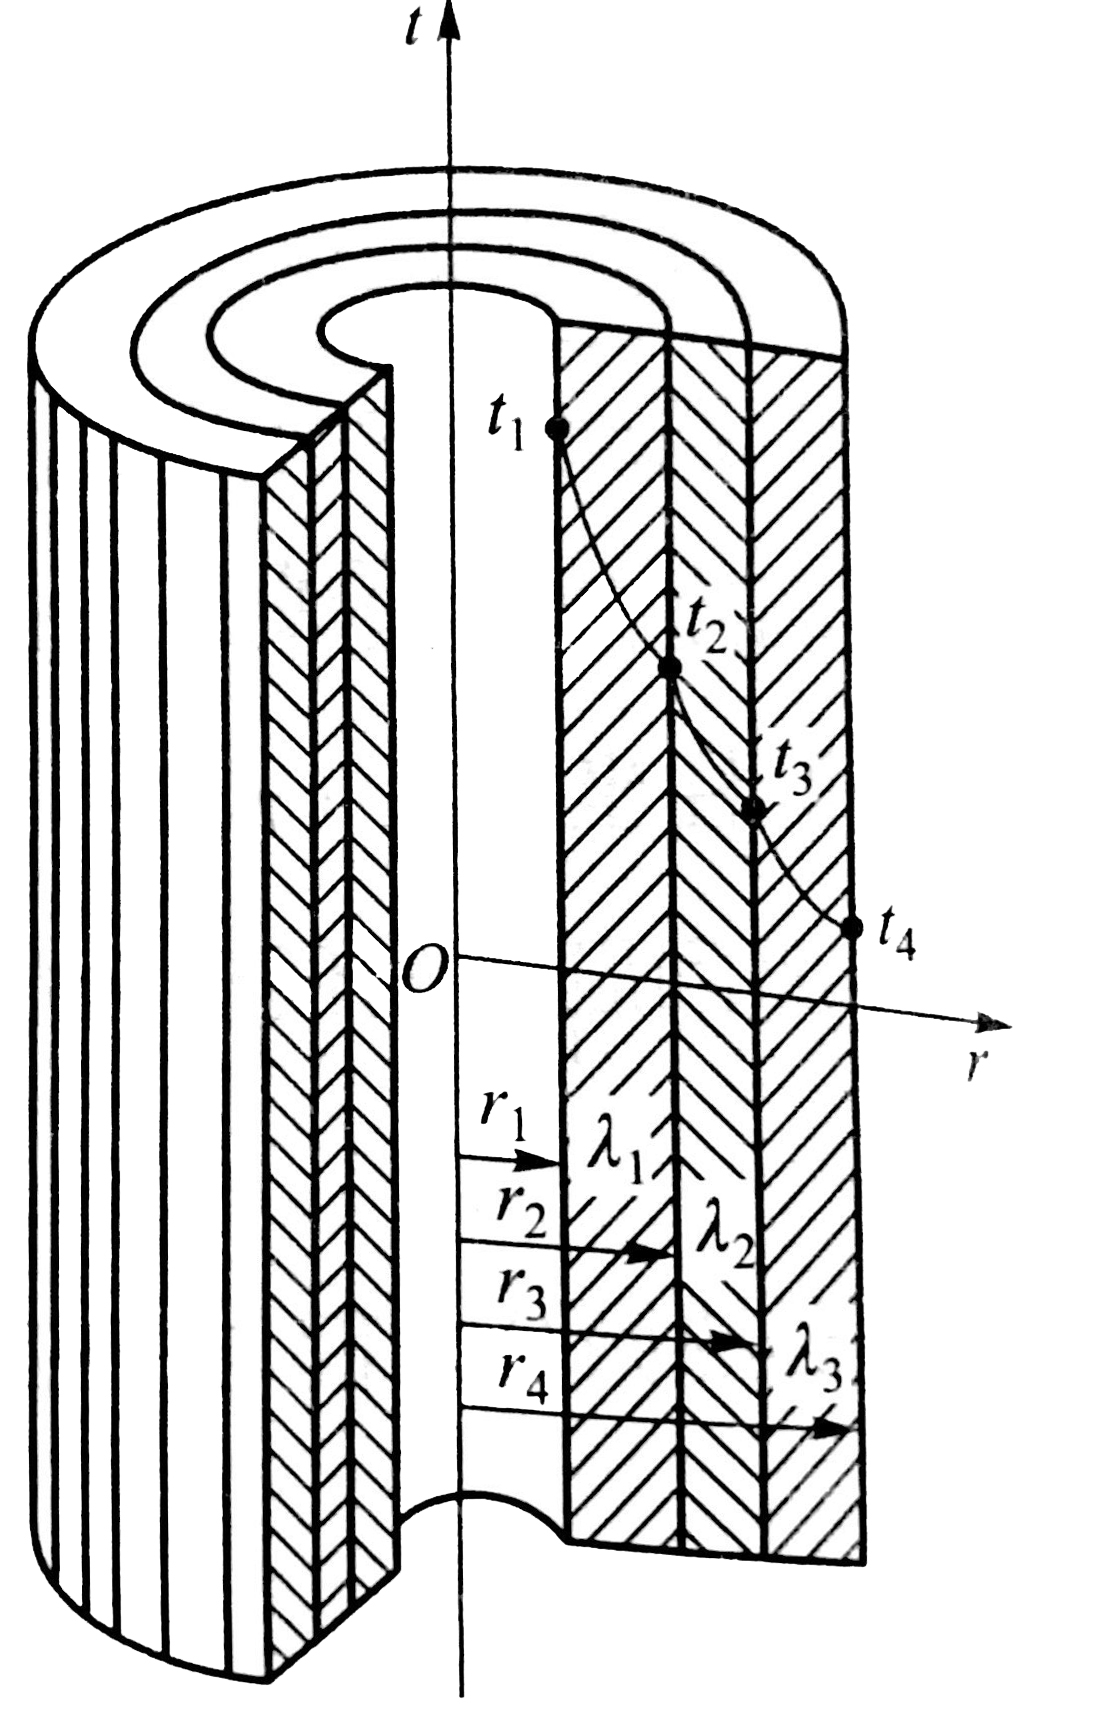
\includegraphics[width=0.4\linewidth]{pic/多圆筒壁.jpeg}
		\vspace*{-1.5em}
		\caption{多圆筒壁的稳态导热}
		\label{多圆筒壁}
	\end{minipage}
\end{figure}
\begin{table}[!htb]
	\centering\setlength{\tabcolsep}{10mm}{
		\begin{tabular}{ccc}
			\toprule
			物理量 &单层圆筒壁的稳态导热 & 单层球壳的稳态导热
\\
			\midrule
			& 	&  \vspace*{-1em}
			\\
			温度分布 & $\displaystyle t = t_1 + \dfrac{t_2 - t_1}{\ln (r_2/r_1)} \ln (r / r_1)$ & $\displaystyle t = t_2 + (t_1 - t_2) \dfrac{1/r - 1/r_2}{1/r_1 - 1/r_2} $ \\[1.5em]
			热流密度 & $\displaystyle q = \dfrac{\lambda}{r} \dfrac{t_1 - t_2}{\ln(r_2/r_1)}$ &$\displaystyle q =\dfrac{\lambda}{r^2}  \dfrac{t_1 - t_2}{1/r_1 - 1/r_2}$ \\[1.5em]
			热流量 &$\varPhi = \dfrac{t_1 - t_2}{\ln(r_2/r_1)/(2 \pi l \lambda)}$ &$\displaystyle \varPhi = \dfrac{t_1 - t_2}{(1/r_1 - 1/r_2)/(4\pi \lambda)}$ \\[1.5em]
			热阻 & $\displaystyle R = \dfrac{\ln(r_2/r_1)}{2\pi l \lambda}$ & $\displaystyle R = \dfrac{1/r_1 - 1/r_2}{4\pi \lambda}$ \\[1.5em]
			\hline
			& 	&  \vspace*{-1.6em}
			\\
			物理量 &多层圆筒壁的稳态导热 & 多层球壳的稳态导热\\
			& 	&  \vspace*{-1.6em}
			\\
			\hline
			& 	&  \vspace*{-1em}
			\\
			热阻 & $\displaystyle R = \sum_{ i =1}^n\dfrac{\ln(r_{i + 1}/r_i)}{2\pi l \lambda_i}$ & $\displaystyle R = \dfrac{1/r_i - 1/r_{i+1}}{4\pi \lambda_i}$ \\[1em]
			\makecell[c]{\\[-0.5em]热流量} &$\varPhi = \dfrac{t_1 - t_{n+1}}{\displaystyle \sum_{ i =1}^n \ln(r_{i+1}/r_{i})/(2 \pi l \lambda_i)}$ &$\displaystyle \varPhi = \dfrac{t_1 - t_{n+1}}{\displaystyle \sum_{ i =1}^n (1/r_i - 1/r_{i+1})/(4\pi \lambda_i)}$ \\[2.5em]
			\bottomrule
		\end{tabular}
		\caption{圆筒壁和球壁的稳态导热规律}
	}
\end{table}

\begin{figure}[!htb]
	\section{通过肋片的导热}
	为了强化传热,可以采取的措施包括:\vspace*{-0.5em}
	\begin{itemize}
		\item 增大温差
\vspace*{-1em}
		\item 减小热阻,包括增大各环节的导热系数、增大传热面积
\vspace*{-0.5em}
	\end{itemize}
{
	\centering
	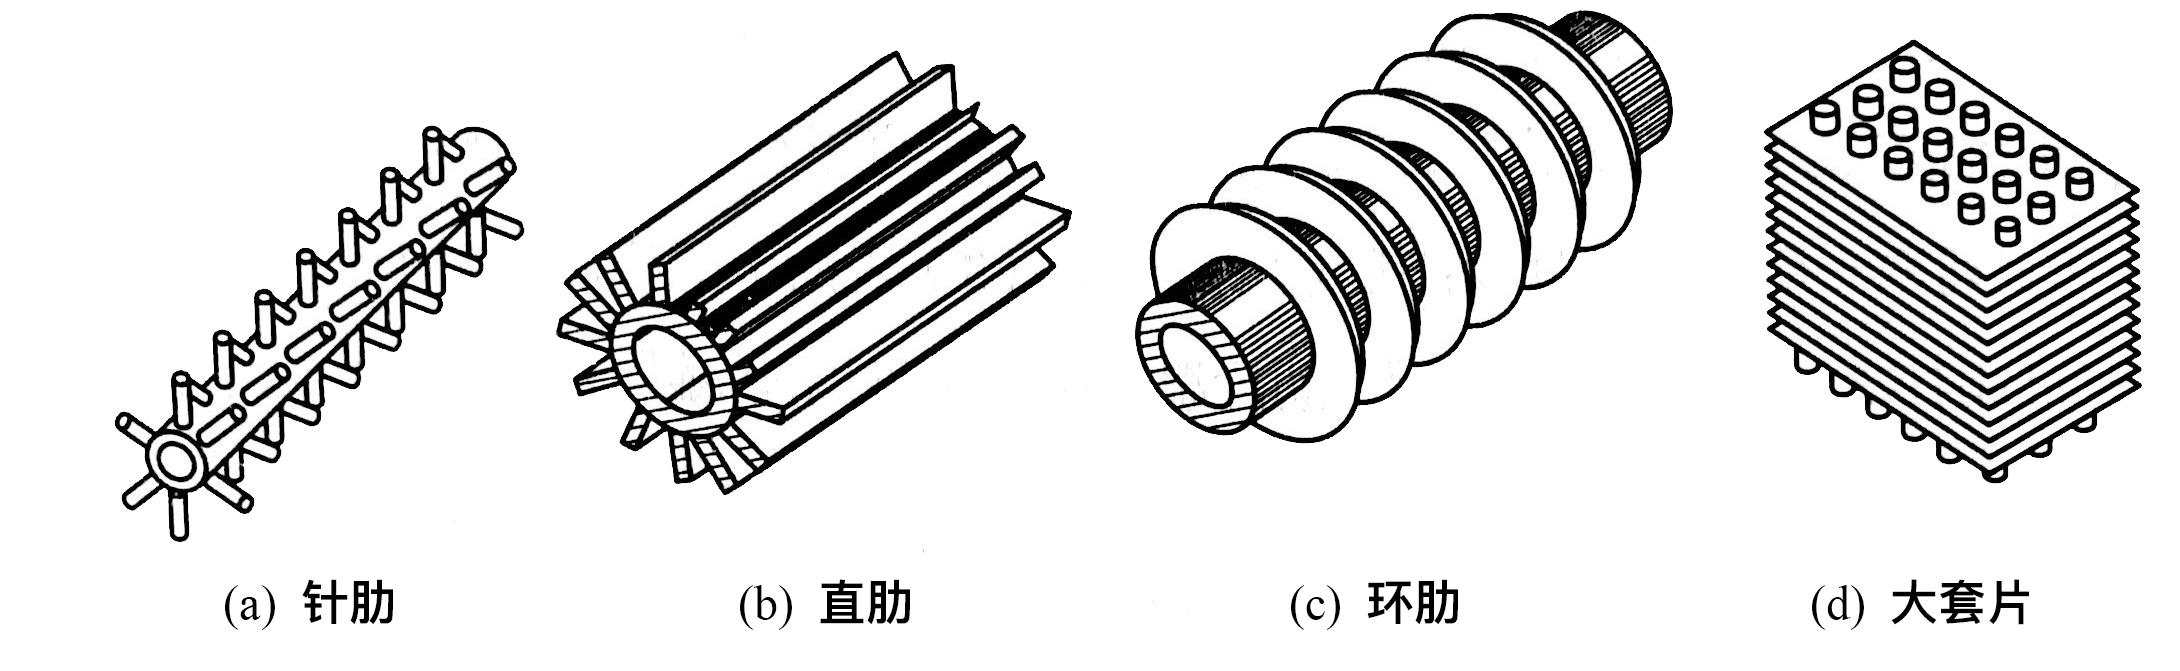
\includegraphics[width=0.75\linewidth]{pic/肋片.jpg}
	\vspace*{-1.5em}
	\caption{肋片的典型结构}
	\label{肋片的典型结构}
}
\vspace*{-2em}
\end{figure}

\newpage
\textbf{工程上强化传热的重要措施是在换热器上加装肋片,增大传热面积。}常见的肋片如图\ref{肋片的典型结构}.
\vspace*{0.5em}

\subsection{等截面直肋的稳态导热
}
\begin{figure}[!htb]
	\vspace*{-1em}
	\centering
	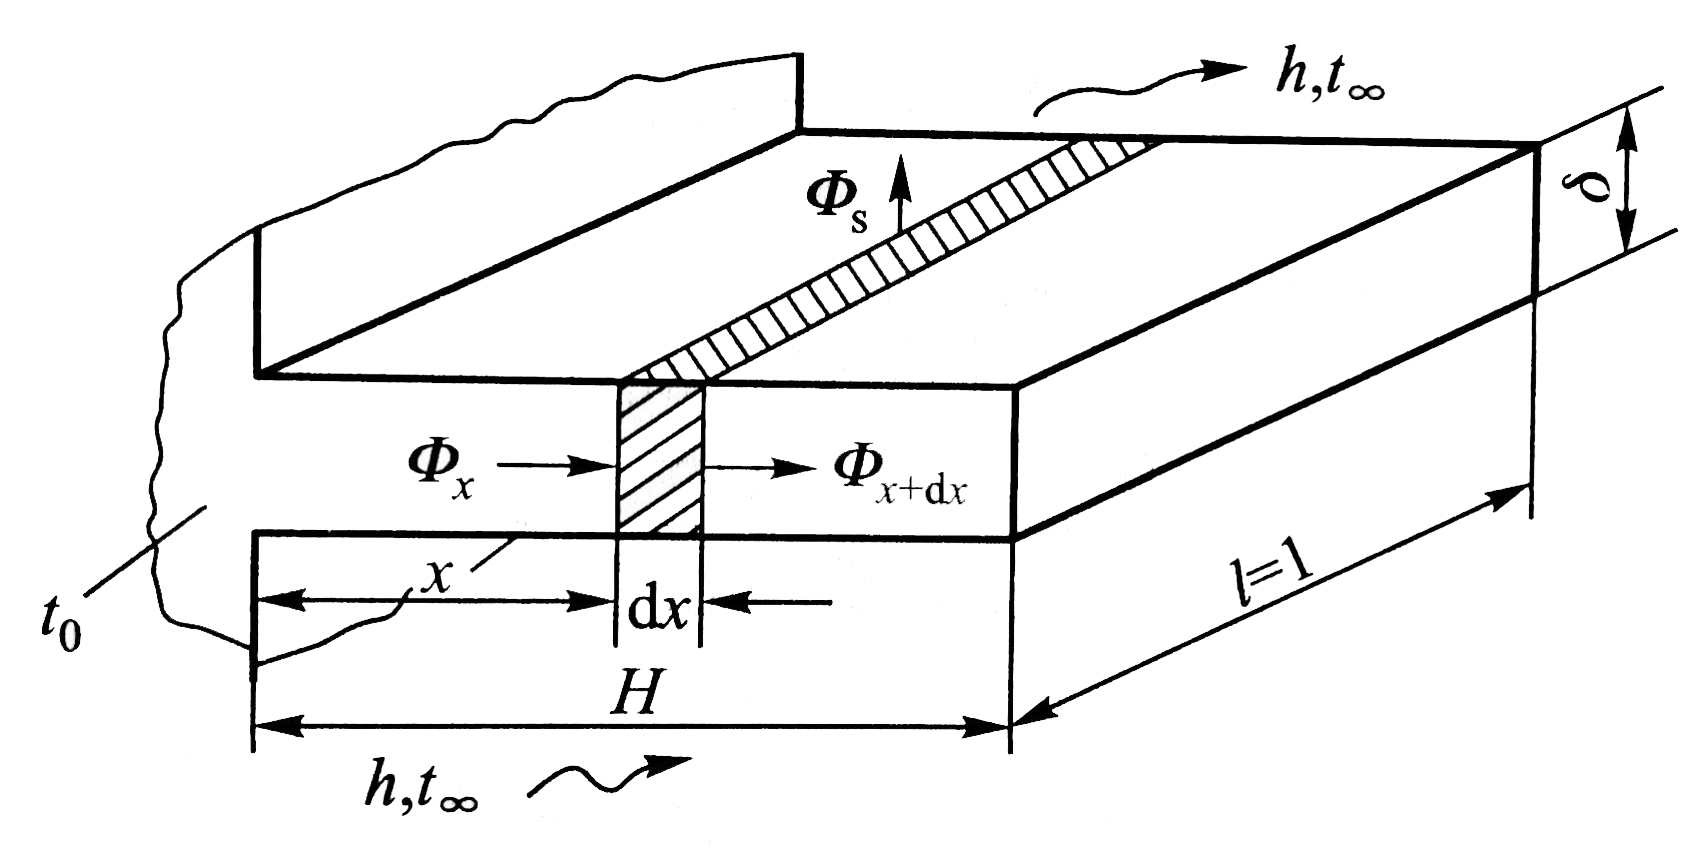
\includegraphics[width=0.5\linewidth]{pic/等截面肋片1.jpeg}
	\vspace*{-1.5em}
	\caption{等截面肋片传热结构图}
	\label{等截面肋片传热结构图}
\end{figure}

\noindent \textbf{1. 物理模型 \& 假设}
\begin{itemize}
	\item 材料的导热系数、表面传热系数及垂直于肋高的截面积均为常数
\vspace*{-0.5em}
	\item 肋片温度沿肋长方向不变
\vspace*{-0.5em}
	\item 肋片温度沿肋厚方向不变
\vspace*{-0.5em}
	\item 肋片顶端近似视为绝热
\end{itemize}
经过假设,可以简化问题为一维稳态常热物性导热问题。

\begin{figure}[!htb]
	\vspace*{-1em}
	\centering
	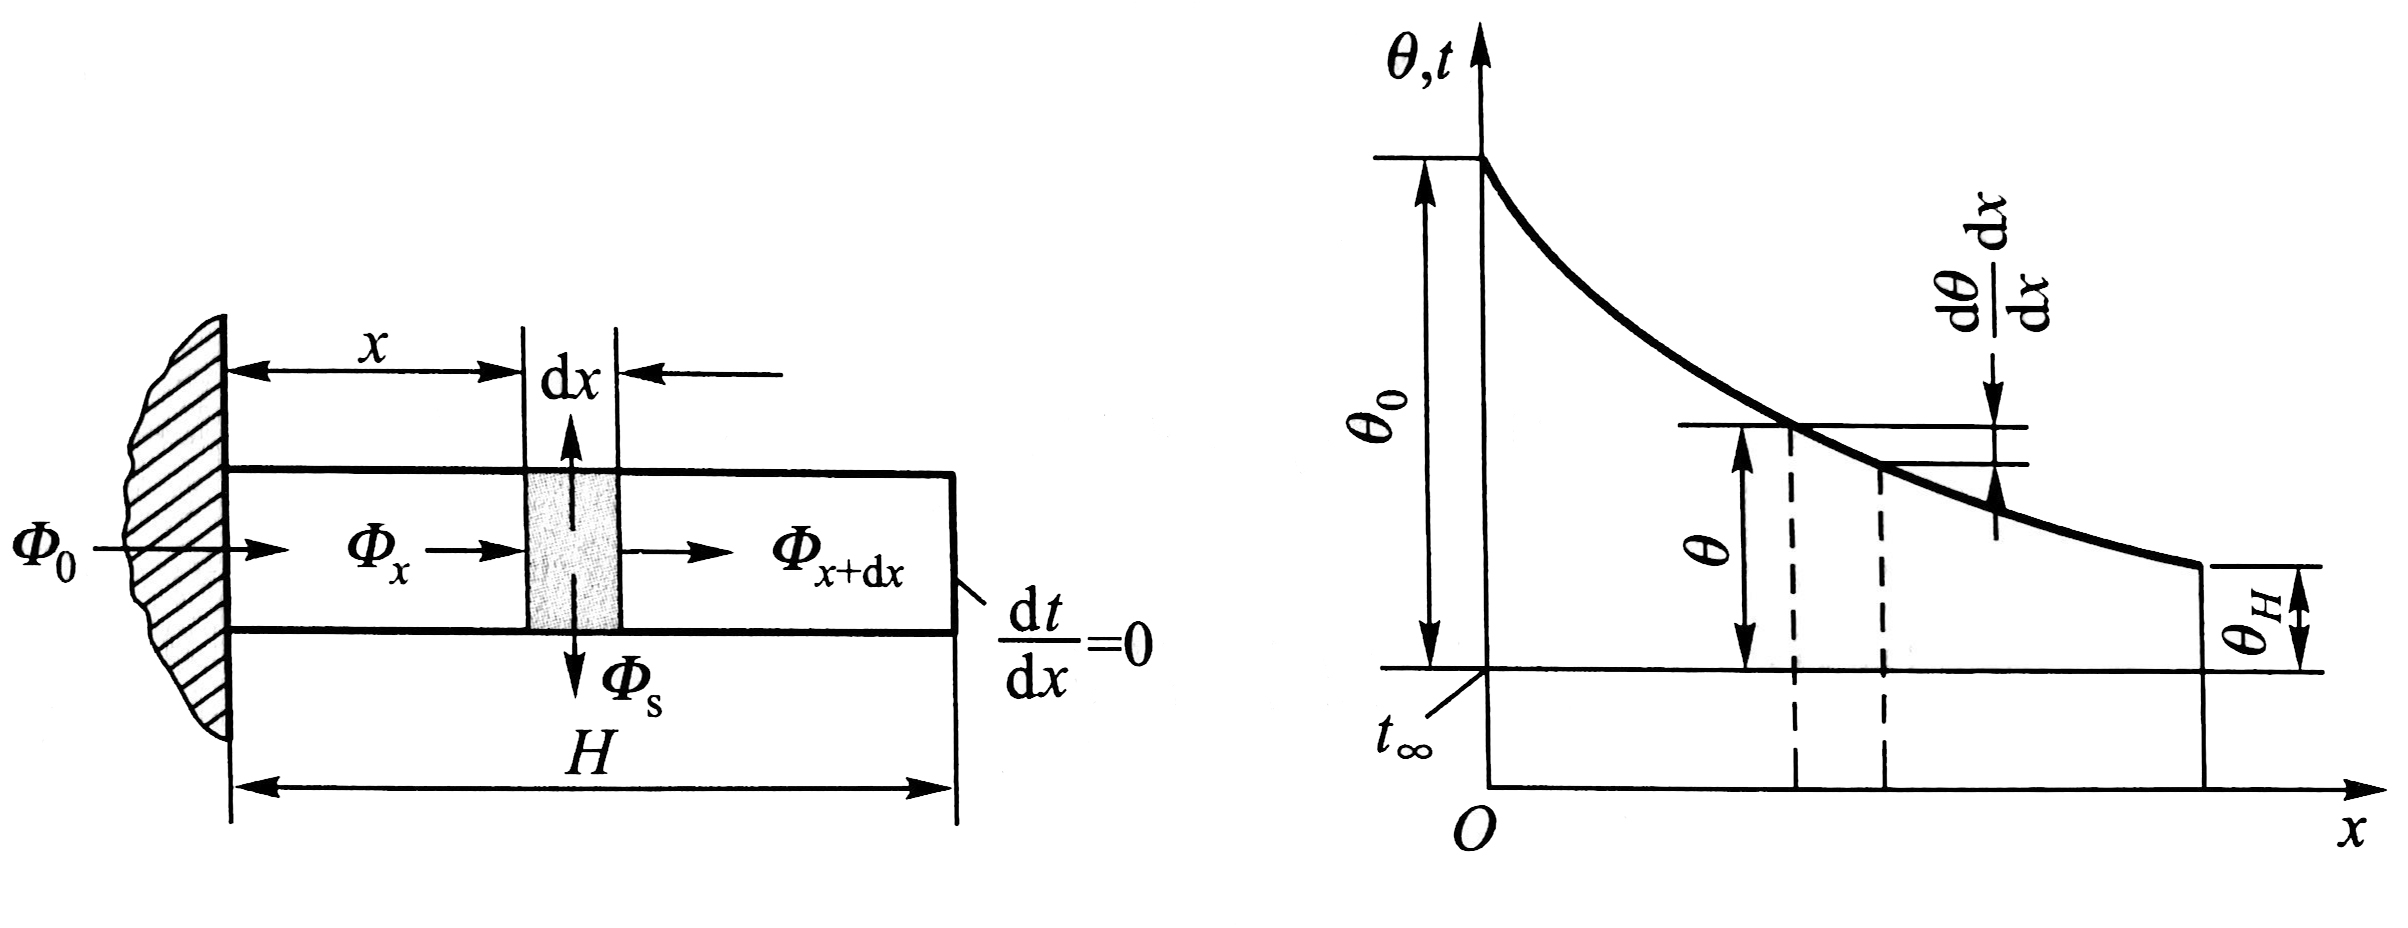
\includegraphics[width=0.8\linewidth]{pic/等截面肋片2.jpeg}
	\vspace*{-1.5em}
	\caption{等截面肋片传热的物理模型}
	\label{等截面肋片传热的物理模型}
\end{figure}
列出定解问题如下
\begin{align}
		\begin{cases}
			\, \dfrac{\d^2 t}{\d x^2}  + \dfrac{\dot{\varPhi}}{\lambda}= 0, & 0< x< H\\
			\, t = t_0, & x = 0\\
			\, \dfrac{\d t}{\d x} = 0, & x = H
		\end{cases}
\end{align}

\noindent \textbf{2. 确定内热源的热流量}

如图\ref{等截面肋片传热的物理模型}所示,取长度为$\d x$的微元段来分析,设参与换热的截面周长为$P$,则表面总散热量为
\begin{align}
	\varPhi_{\text{s}} = (P \d x) h (t - t_\infty)
\end{align}
其对应的微元体积为$\d V = A_{\text{c}} \d x$,由热源强度$\dot{\varPhi}$的定义,
\begin{align}
	\dot{\varPhi} = \dfrac{-\varPhi_{\text{s}}}{\d V} = -\dfrac{h P (t - t_\infty)}{A_{\text{c}}}
\end{align}

\noindent \textbf{3. 分析求解}

得到最终的定解问题
\begin{align}
	\begin{cases}
		\, \dfrac{\d^2 t}{\d x^2}  = \dfrac{h P (t - t_\infty)}{A_{\text{c}}\lambda}, & 0< x< H\\
		\, t = t_0, & x = 0\\
		\, \dfrac{\d t}{\d x} = 0, & x = H
	\end{cases}
\end{align}
令$\theta = t_0 - t_\infty, m = \sqrt{\dfrac{h P}{A_{\text{c}}\lambda}}$,则微分方程改写为
\begin{align}
	\dfrac{\d^2 \theta}{\d x^2} - m^2 \theta = 0
\end{align}
由高等数学常微分方程求解理论,得到方程通解
\begin{align}
	\theta = C_1 \e^{mx} + C_2 \e^{-mx}
\end{align}

考虑边界条件,得到等截面肋片的温度分布为
\begin{align}
	\theta = \theta_0 \dfrac{\ch \big[m(x - H)\big]}{\ch (mH)}
\end{align}
其中,$\ch$代表双曲余弦函数。
\vspace*{0.5em}

\noindent \textbf{4. 求解结果}


	\begin{figure}[!htb]
		\begin{minipage}{0.73\linewidth}
			\begin{itemize}
				\item 由于由肋片散入外界的热量都必须通过肋根截面,故此热量为:
				\begin{align}
					\varPhi_{x = 0} = - \lambda A_{\text{c}}\left(\dfrac{\d \theta}{\d x}\right)_{x = 0} = \lambda A_{\text{c}} \theta_0 (-m) \text{th}(mH)
				\end{align}
				
				\item 肋实际散热量与假设整个肋表面处于肋基温度下的散热量之比称为\dy[肋效率]{LXL}
				\begin{align}
					\eta_{\text{f}} = \dfrac{\lambda A_{\text{c}} \theta_0 (-m) \text{th}(mH)}{h P H \theta_0} = \dfrac{\text{th}(mH)}{mH}
				\end{align}
				\item 肋面(包括肋基和所有肋片)实际散热量与假设整个肋面表面处于肋基温度下的散热量之比称为\dy[肋面总效率]{LMZXL},如图\ref{总肋面效率图}.
				\begin{align}
					\eta_0 = \dfrac{hA_{\text{r}}(t_0 - t_{\infty}) + hA_{\text{f}}(t_0 - t_{\infty})\eta_\text{f}}{h(A_{\text{r}}+A_{\text{f}})(t_0 - t_{\infty}) } =\dfrac{A_{\text{r}} + A_{\text{f}}\eta_\text{f}}{A_{\text{r}}+A_{\text{f}} }  > \eta_{\text{f}} 
				\end{align}
		\end{itemize}
		\end{minipage}
		\begin{minipage}{0.27\linewidth}
			\vspace*{-0.5em}
			\centering
			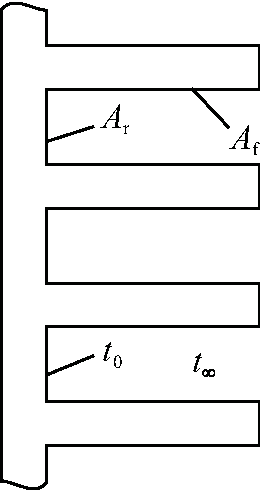
\includegraphics[width=0.6\linewidth]{pic/总肋面效率.pdf}
			\vspace*{-1.5em}
			\caption{局部肋面}
			\label{总肋面效率图}
		\end{minipage}
	\end{figure}
	

\section{具有内热源的一维导热问题}
\subsection{具有内热源的平板导热}
\noindent \textbf{1. 定解问题}

列出方程及边界条件如下
\begin{align}
	\begin{cases}
		\, \dfrac{\d^2 t}{\d x^2} + \dfrac{\dot{\varPhi}}{\lambda} = 0, & 0< x < \delta\\[0.5em]
		\, \dfrac{\d t}{\d x} = 0, & x = 0\\[0.5em]
		\, - \lambda \dfrac{\d t}{\d x} = h(t - t_\f), & x = \delta
	\end{cases}
\end{align}

\noindent \textbf{2. 求解各物理量}

解常微分方程,可以得到\vspace*{-0.5em}
\begin{itemize}
	\item 温度分布\vspace*{-1em}
	\begin{align}
		t = \dfrac{\dot{\varPhi}}{2 \lambda} \left(\delta^2 - x^2 \right) + \dfrac{\dot{\varPhi}\delta }{h}+ t_\f
	\end{align}
	\vspace*{-1em}
	\item 热流密度\vspace*{-1em}
	\begin{align}
		q = - \lambda \dfrac{\d t}{\d x} = \dot{\varPhi }x
	\end{align}
\vspace*{-1em}
\end{itemize}

\noindent \textbf{3. 特点}\vspace*{-0.5em}
\begin{itemize}
	\item 温度分布不再是直线而是抛物线\vspace*{-0.5em}
	\item 热流密度不再是常数
\end{itemize}

\noindent \textbf{4. 给定壁面温度的情形}

由于给定壁面温度的情形可视为表面传热系数趋于无穷大从而流体温度等于壁面温度,因此由前述温度分布可得给定两侧壁面温度均为$t_\w$时平板的温度分布为:
\begin{align}
	t = \dfrac{\dot{\varPhi}}{2 \lambda} \left(\delta^2 - x^2 \right) + t_\w
\end{align}


\subsection{具有内热源的圆柱体导热}
\noindent \textbf{1. 定解问题}

列出方程及边界条件如下
\begin{align}
	\begin{cases}
		\, \dfrac{1}{r}\dfrac{\d}{\d r}\left(r \dfrac{\d t}{\d r}\right)+ \dfrac{\dot{\varPhi}}{\lambda} = 0, & 0< r < r_1 \\[0.5em]
		\, \dfrac{\d t}{\d x} = 0, & r = 0\\[0.5em]
		\, t = t_1, & r = r_1
	\end{cases}
\end{align}

\noindent \textbf{2. 求解各物理量}

解常微分方程,可以得到温度分布
	\begin{align}
		t = \dfrac{1}{4} \dfrac{\dot{\varPhi}}{\lambda}\left(r_1^2 - r^2\right)+ t_1
	\end{align}
圆柱体中的最高温度出现在圆心处,为
\begin{align}
	t_{\max} =  \dfrac{1}{4} \dfrac{\dot{\varPhi}r_1^2}{\lambda} + t_1
\end{align}






\section{多维稳态导热的求解}

\subsection{稳态导热求解方法概述}
\begin{itemize}
	\item \dy[分析法]{FXF}
\\
	\hspace*{2em} 通过数学分析方法求解定解条件下的导热微分方程来获得温度场函数
\vspace*{-0.5em}
	
	\item \dy[数值法]{SZF}
\\
	\hspace*{2em} 通过计算机获得某个计算条件下物体中代表性空间点上的温度值
\vspace*{-0.5em}
	
	\item \dy[比拟法]{BNF}
\\
	\hspace*{2em} 通过比较容易测量的电势场来获得温度场
\end{itemize}

\subsection{求解稳态导热的分离变量法}

\noindent \textbf{1. 定解问题}

列出方程及边界条件如下
\begin{align}
	\begin{cases}
		\dfrac{\partial^2 t}{\partial x^2} + \dfrac{\partial^2 t}{\partial x^2}  = 0 \quad 0<x<a,\, 0<y<b \\[0.5em]
		\, t(0,y) = t_1\\
		\, t (a, y) = t_1\\
		\, t(x, 0) = t_1\\
		\, t(s,b) = t_2
	\end{cases}
\end{align}
引入无量纲过余温度
\begin{align}
	\varTheta = \dfrac{t - t_1}{t_2 - t_1}
\end{align}
则定解问题变为
\begin{align}
	\begin{cases}
		\dfrac{\partial^2 t}{\partial x^2} + \dfrac{\partial^2 t}{\partial x^2}  = 0 \quad 0<x<a,\, 0<y<b \\[0.5em]
		\, \varTheta(0,y) = 0\\
		\, \varTheta (a, y) = 0\\
		\, \varTheta(x, 0) = 0\\
		\, \varTheta(s,b) = 1
	\end{cases}
\end{align}
\noindent \textbf{2. 求解物理量}

由分离变量法解偏微分方程,可以得到分析解
\begin{align}
	\varTheta = \dfrac{2}{\pi} \sum_{ n =1}^\infty \dfrac{(-1)^{n+1} + 1}{n} \sin \dfrac{n \pi x}{a} \dfrac{\sh(n \pi y /a)}{\sh(n \pi b / a)}
\end{align}

\subsection{计算导热量的形状因子法
}
\textcolor{red}{若只需求解导热量,且物体位于两个定温边界之间,则可采用形状因子法。}\index{XZYZF@形状因子法}

一维问题中,两个等温面间导热热流量总可以表示为以下统一形式:
\begin{align}
	\varPhi = \lambda S (t_1 - t_2)
	\label{形状因子法}
\end{align}
二维和三维问题中公式\eqref{形状因子法}也成立,其中S与导热物体的形状及大小有关,称为\dy[形状因子]{XZYZ}。对于工程中常见的许多复杂结构的导热问题\vspace*{-0.5em}
\begin{itemize}
	\item 已经通过分析方法或数值方法解出了其形状因子的表达式
\vspace*{-0.5em}
	\item 可查表得到形状因子,求解导热热流量,进而求解导热量
\end{itemize}











